% Figures and text for the "Conducting the review" section.
% Requires \usepackage{graphicx}. Put the figures/ folder next to your main .tex file.

The final corpus contains 394 primary studies: 285 on multimodal fake news detection and 109 on multimodal deepfake detection. Figures~\ref{fig:years}--\ref{fig:modalities} describe the corpus by publication year, venue type, publisher, first-author country and modality.

\begin{figure}[t]
  \centering
  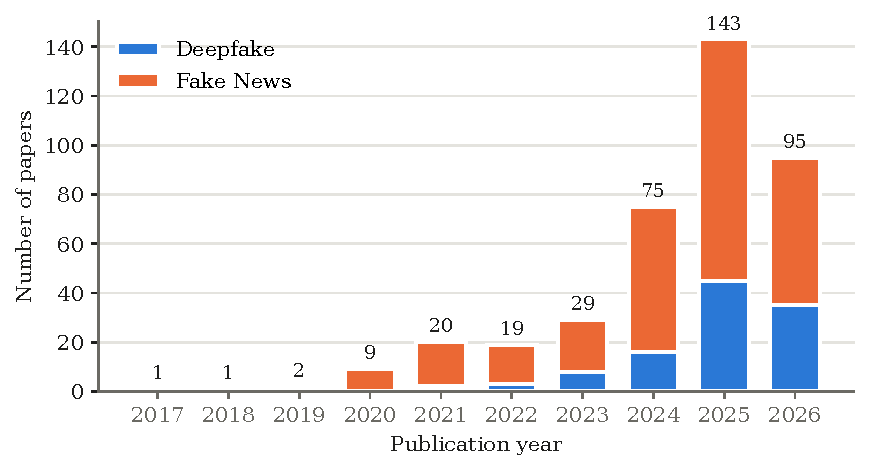
\includegraphics[width=\linewidth]{figures/fig_papers_per_year.pdf}
  \caption{Number of selected papers per publication year, split into deepfake and fake news detection.}
  \label{fig:years}
\end{figure}

\textbf{Publication trend.} Research on multimodal detection has grown quickly (Fig.~\ref{fig:years}). Before 2023, the field produced at most 20 selected papers per year. The count rose to 75 in 2024 and 143 in 2025, and 313 of the 394 papers (79.4\%) were published from 2024 onwards. Deepfake detection grew fastest, from 8 papers in 2023 to 45 in 2025. This growth coincides with the spread of accessible generative models. The 2026 count (95) covers only part of the year, so it should not be read as a decline.

\begin{figure}[t]
  \centering
  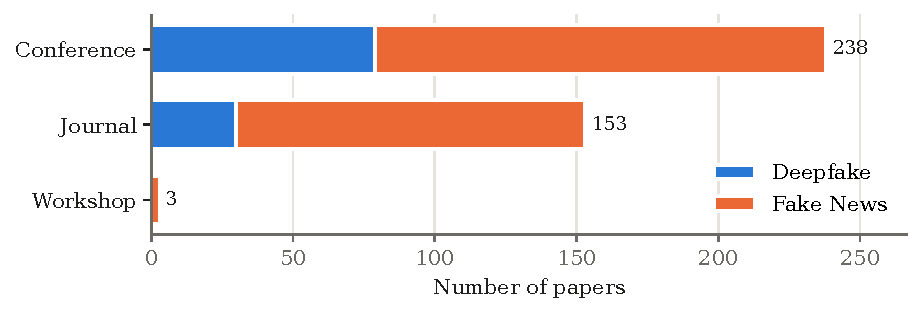
\includegraphics[width=\linewidth]{figures/fig_venue_type.pdf}
  \caption{Distribution of the selected papers by venue type.}
  \label{fig:venue}
\end{figure}

\textbf{Venue type.} Conference papers form the majority, with 238 papers (60.4\%), followed by 153 journal articles (38.8\%) and 3 workshop papers (Fig.~\ref{fig:venue}). The split differs by topic. Deepfake detection appears mostly at conferences (79 of 109 papers), while fake news detection is more balanced (159 conference and 123 journal papers). This suggests that audio-visual deepfake detection is a younger, fast-moving area that relies on conferences for rapid dissemination.

\begin{figure}[t]
  \centering
  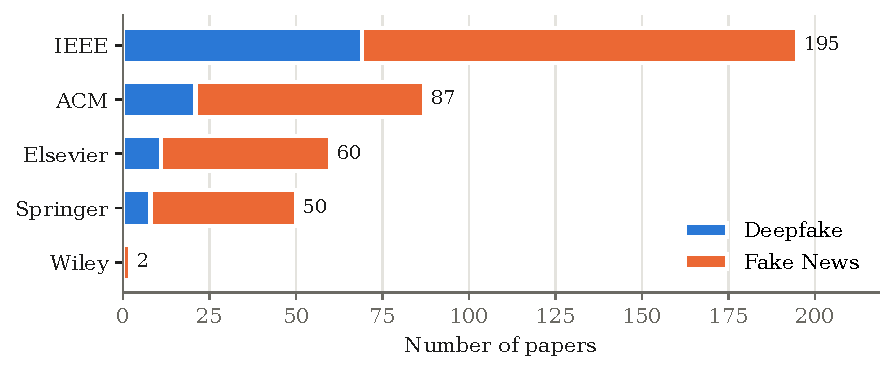
\includegraphics[width=\linewidth]{figures/fig_publisher.pdf}
  \caption{Distribution of the selected papers by publisher.}
  \label{fig:publisher}
\end{figure}

\textbf{Publishers.} IEEE is the main venue, with 195 papers (49.5\%), followed by ACM (87), Elsevier (60), Springer (50) and Wiley (2) (Fig.~\ref{fig:publisher}). IEEE also hosts most deepfake detection papers (69 of 109).

\begin{figure}[t]
  \centering
  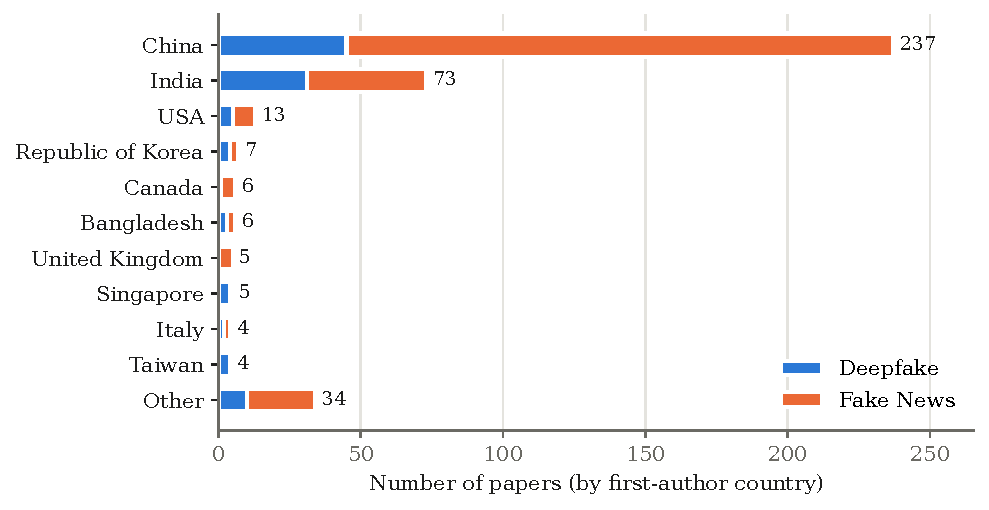
\includegraphics[width=\linewidth]{figures/fig_countries.pdf}
  \caption{Top ten first-author countries of the selected papers. Remaining countries are grouped as ``Other''.}
  \label{fig:countries}
\end{figure}

\textbf{Geographic distribution.} Based on the first author's affiliation, the corpus is highly concentrated (Fig.~\ref{fig:countries}). China accounts for 237 papers (60.2\%) and India for 73 (18.5\%), together almost 80\% of the corpus. The USA follows with 13 papers, and no other country exceeds 7. China's share is driven by fake news detection, much of it evaluated on the Chinese Weibo dataset, while deepfake work is spread more evenly across countries. This concentration means that languages, platforms and contexts outside China and India remain under-studied.

\begin{figure}[t]
  \centering
  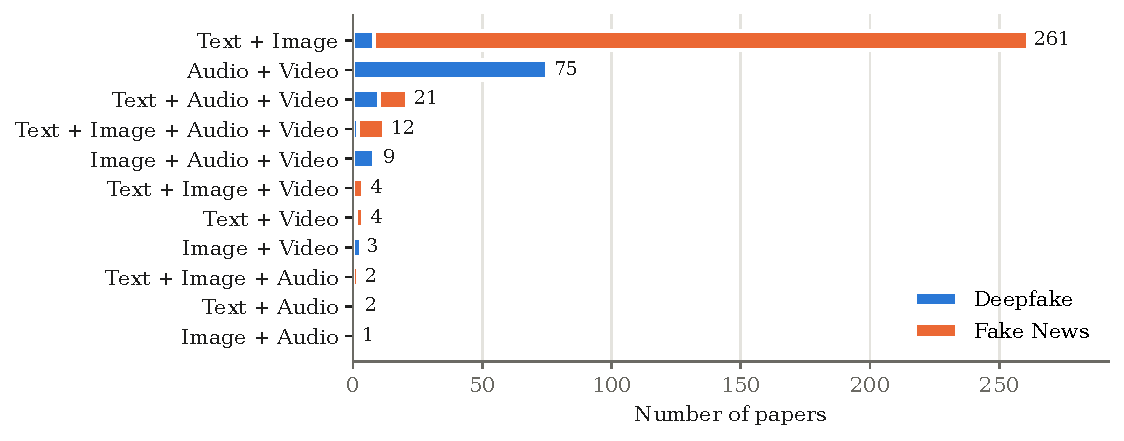
\includegraphics[width=\linewidth]{figures/fig_modalities.pdf}
  \caption{Modality combinations addressed by the selected papers.}
  \label{fig:modalities}
\end{figure}

\textbf{Modalities.} Two combinations dominate (Fig.~\ref{fig:modalities}). Text~+~image covers 261 papers (66.2\%), almost all on fake news detection in social media posts. Audio~+~video covers 75 papers (19.0\%), all on deepfake detection. Only 12 papers use all four modalities, and combinations involving audio with text or image are rare. Joint analysis of all modalities therefore remains an open direction.
